\section{Lambda}
Ao todo o \texttt{visitor} responsável por pesquisar a adoção de \textit{Lambda} encontrou somente 824 caso de uso. Distribuídos em 365 arquivos o que leva a acreditar que tal característica não esta sendo tão relevante quanto sua expectativa de lançamento. Onde somente 2 casos não estão envolvidos em testes unitários, os demais 824 estão sendo empregados no desenvolvimento de testes unitários conforme exibido pela figura: \ref{fig:AdocaoLambda}. Vale ressaltar que somente duas únicas ocorrências de lambda foram encontradas no projeto Jetty versão 9.3.2 nos fontes \textit{PathMap.java} e \textit{RegexSet.java}.\\

\begin{figure}[h]
	\center
	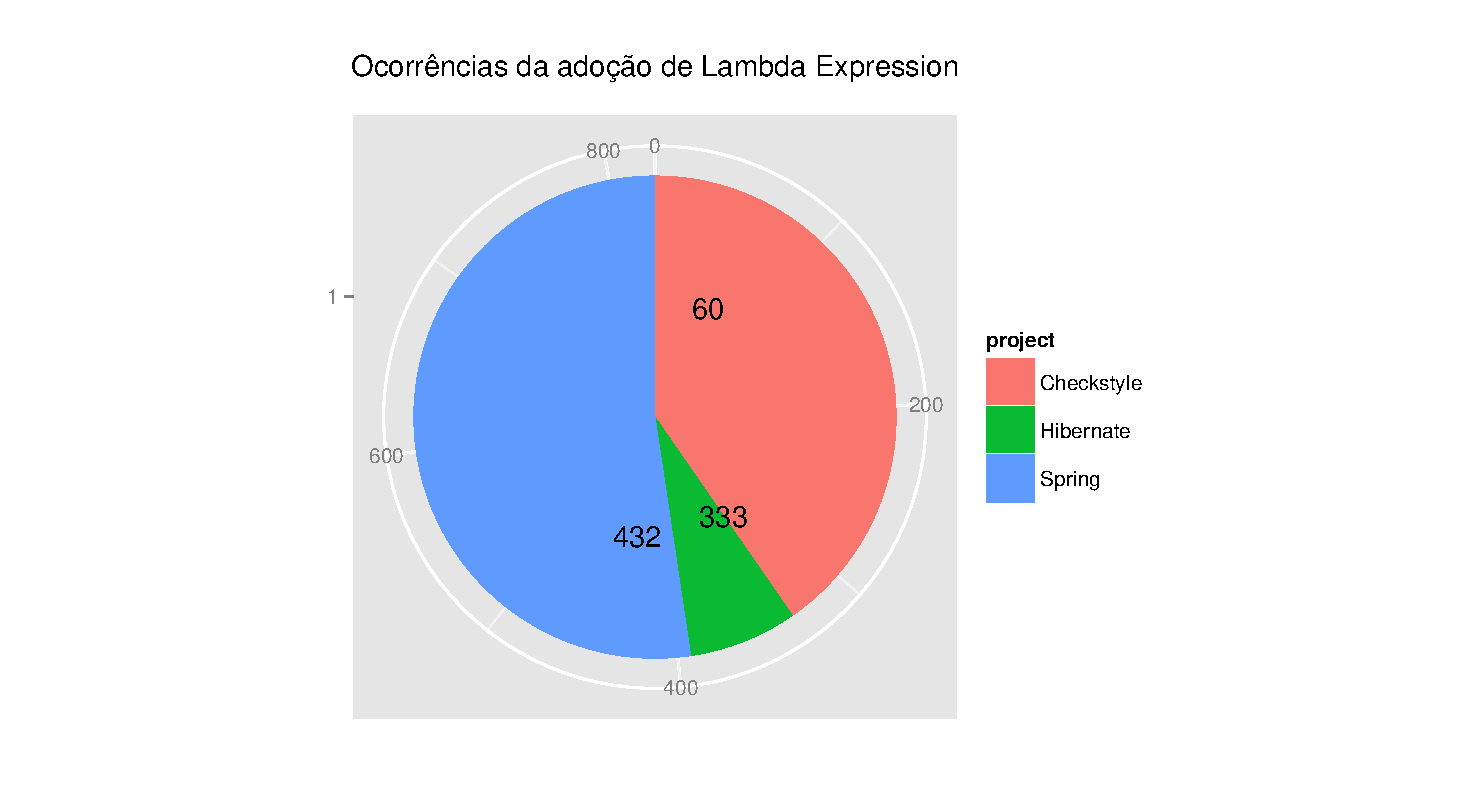
\includegraphics[scale=0.5]{Imagens/AdocaoLambdaTestes}
	\label{fig:AdocaoLambda}
	\caption{Adoção de \textit{Lambda} em testes unitários.}
\end{figure}



\subsection{Oportunidades de Aplicar Lambda}
Entretanto foram encontradas 2618 caso de possível utilização de \textit{Lambda Expression} distribuído em 1635 oportunidades sobre o padrão \textit{exists} onde um \textit{loop} que itera \textit{Collections} para verificar se um elemento existe. E 983 que utilizam o padrão \textit{filter} onde um \textit{loop} que itera uma \textit{Collection} retornar uma outra \textit{Collection} com os elementos dado um filtro. Onde em ambos os casos podem ser migrados para \textit{Lambda} através da \textit{Inteface Stream}.


 %estas oportunidades foram baseados em padrões simples como aplicação de uso de filter e map. Também foram pesquisadas oportunidades de encontrar \textit{anonymous inner class} que possam se migradas para \textit{Lambda}.
A figura: \ref{fig:ocorenciasFilterExists}, exibe a distribuição do padrão \textit{exists} e \textit{filter} encontrados pelos \textit{visitors}.

\begin{figure}[h]
	\center
	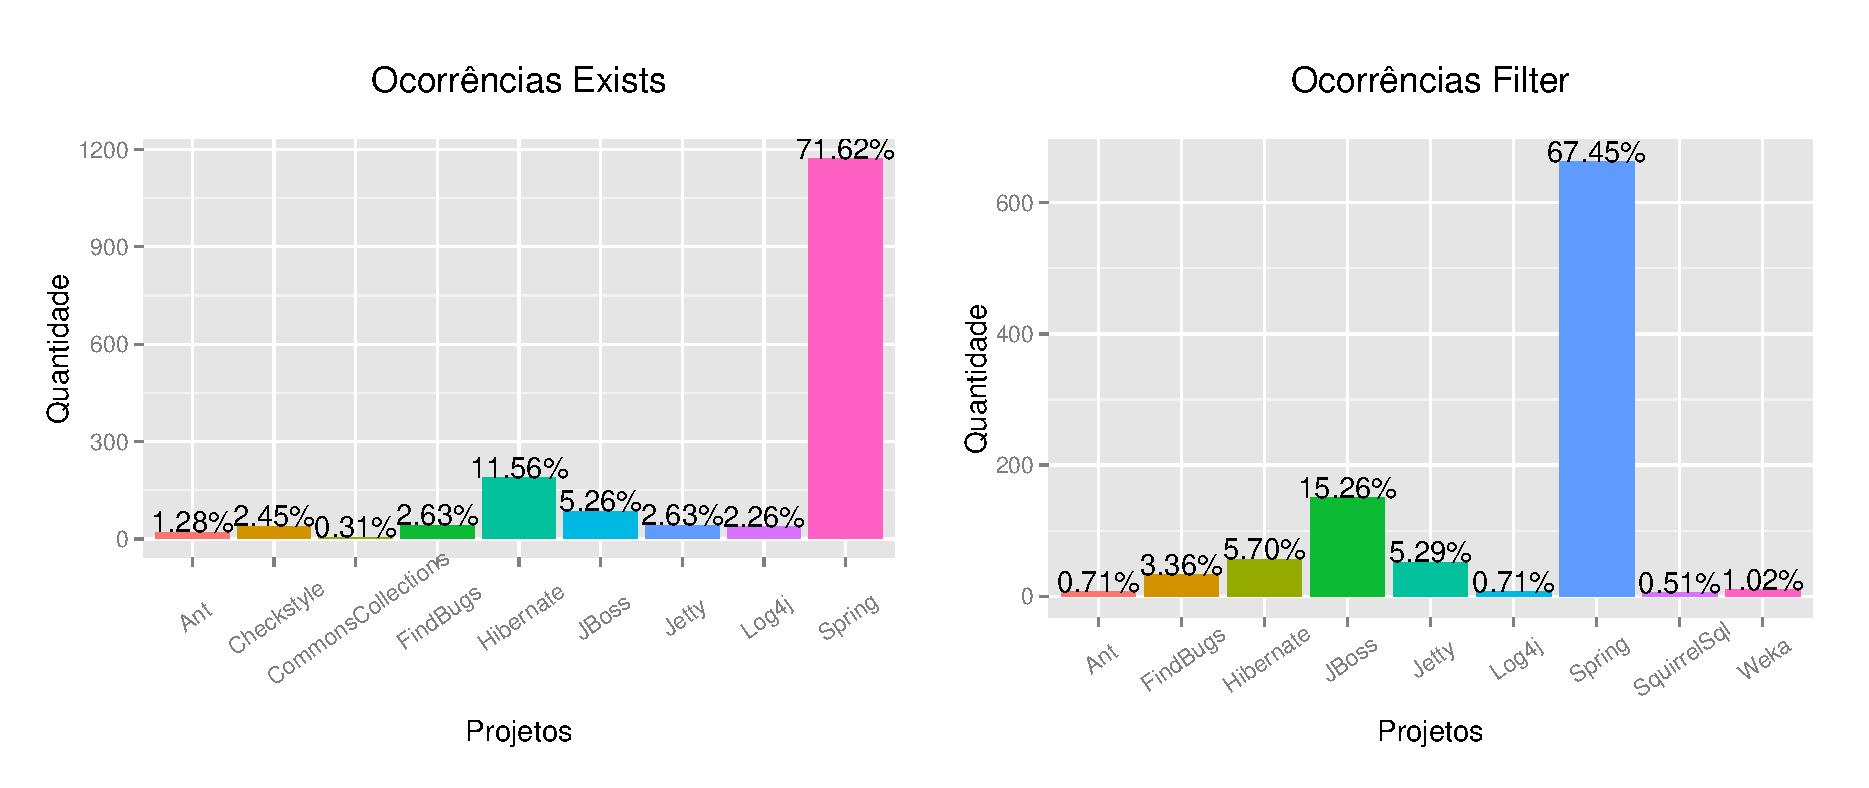
\includegraphics[scale=0.5]{Imagens/ocorrenciasFilter_Exists}
	\label{fig:ocorenciasFilterExists}
	\caption{Ocorrências de Filter e Exists nos Projetos.}
\end{figure}

Uma ênfase mais minuciosa sobre o Spring para demonstrar como suas \textit{releases} tem distribuído essas ocorrências pois pode-se constatar que com 67.45\%, 663 casos,  de \textit{Filter} e com 71.62\%, 1170 casos, de Exists é o projeto que contém mais ocorrências destas características a Figuras: \ref{fig:filterSpring} e \ref{fig:existsSpring}.

\begin{figure}[h]
	\center
	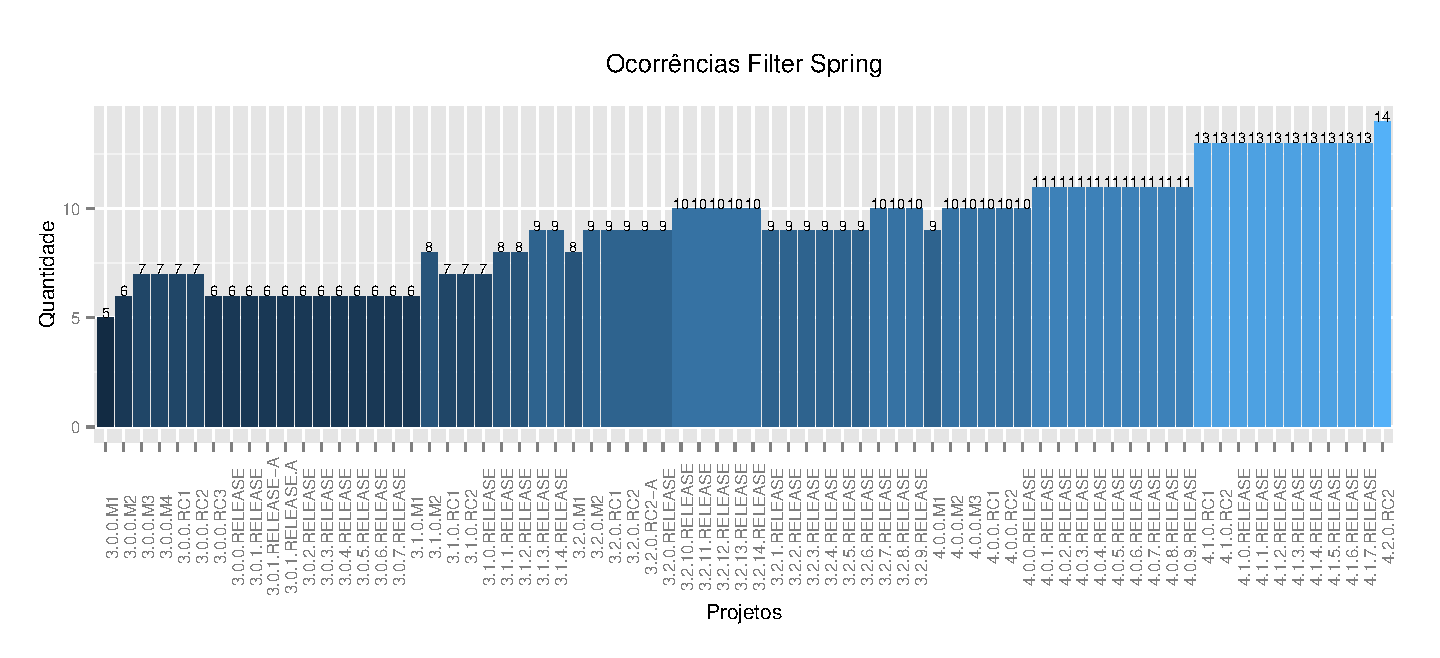
\includegraphics[scale=0.7]{Imagens/ocorrenciasFilterSpring}
	\label{fig:filterSpring}
	\caption{Ocorrências de Filter nas Versões do Spring.}
\end{figure}


\begin{figure}[h]
	\center
	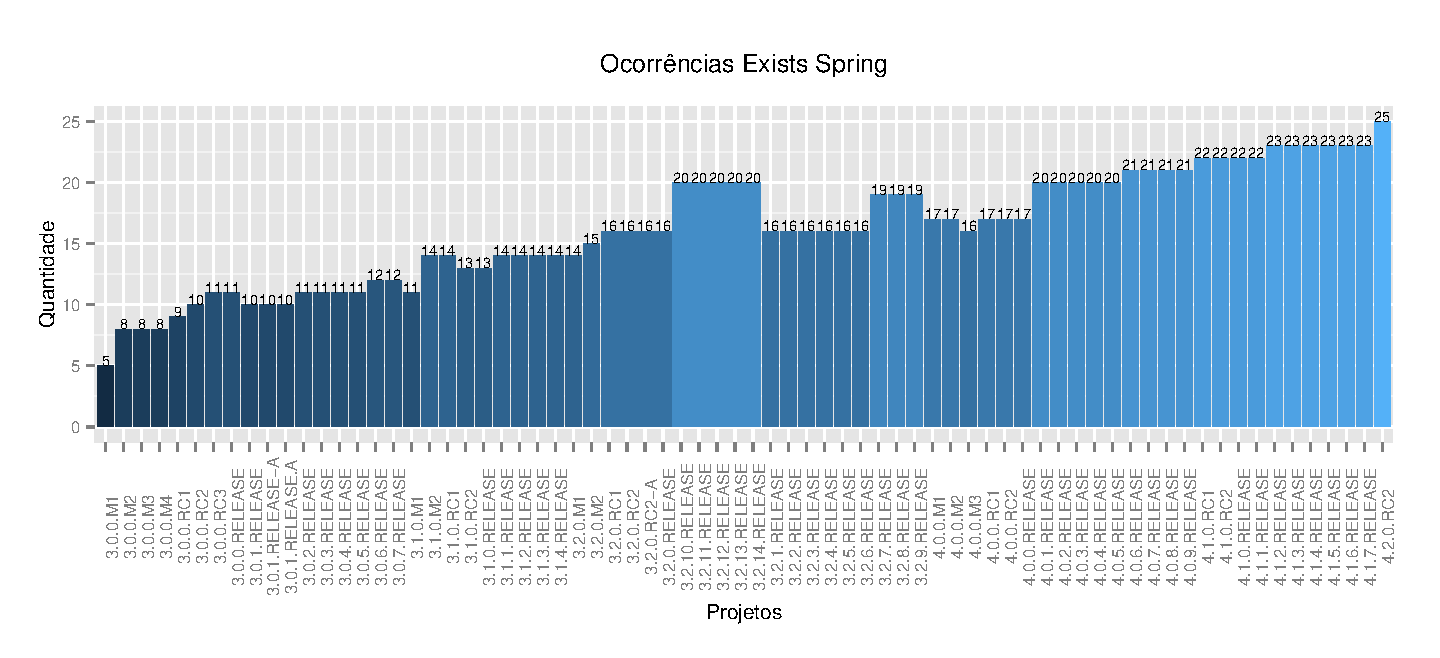
\includegraphics[scale=0.7]{Imagens/ocorrenciasExistsSpring}
	\label{fig:existsSpring}
	\caption{Ocorrências de Exists nas Versões do Spring.}
\end{figure}